\section{El litio como un elemento estratégico}
El litio es un elemento clave para sectores económicos muy importantes porque sus propiedades lo hacen muy apropiado para diferentes aplicaciones. En dispositivos de almacenamiento de energía eléctrica son útiles su extremo potencial estándar de reducción (-3.045~V, el menor para los elementos de la tabla periódica) y su baja masa atómica, que provee una excelente relación carga/masa \citep{Bagotsky2006}. Tiene la capacidad calorífica específica más alta de los elementos sólidos (3.489~J~mol\mnn\ a 20$^o$C), y un muy alto coeficiente de expansión térmica, por lo que provee resistencia a cerámicos y vidrios frente a cambios bruscos de temperatura \citep{Hart1973}. El litio también es utilizado ampliamente en la elaboración de grasas y lubricantes especiales (en forma de sales líticas de ésteres de ácidos grasos), en producción de aluminio aeroespacial (para lo que se usa litio metálico de elevada pureza), en la elaboración de polvos fundentes, y en la deshumidificación de aire.

\begin{figure}[htbp]
    \subbottom{\begin{picture}(500,210)
               \put(5, 0){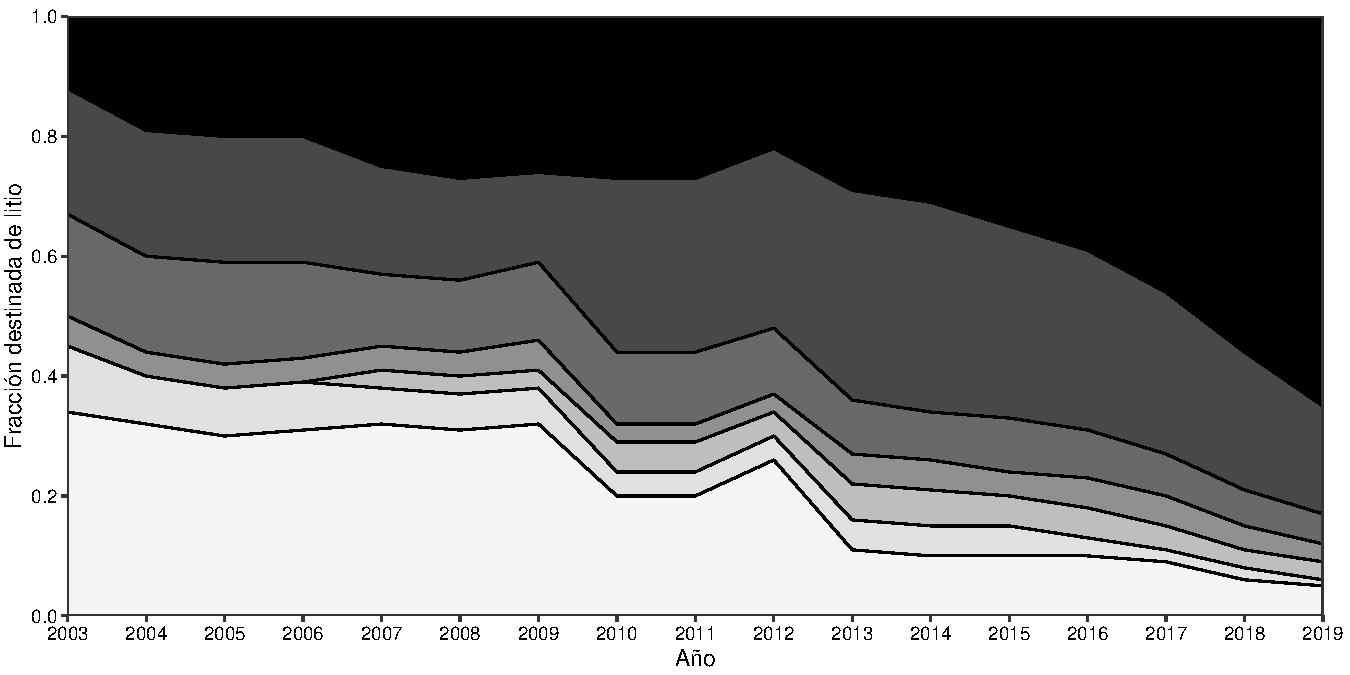
\includegraphics[width=0.986\textwidth,trim={0 0.85cm 0 0}, clip]{chap2/images/usesRel.pdf}}
               \put(2, 202){\large a)}
               \end{picture}}\\%
    \subbottom{\begin{picture}(500,230)
               \put(0, 0){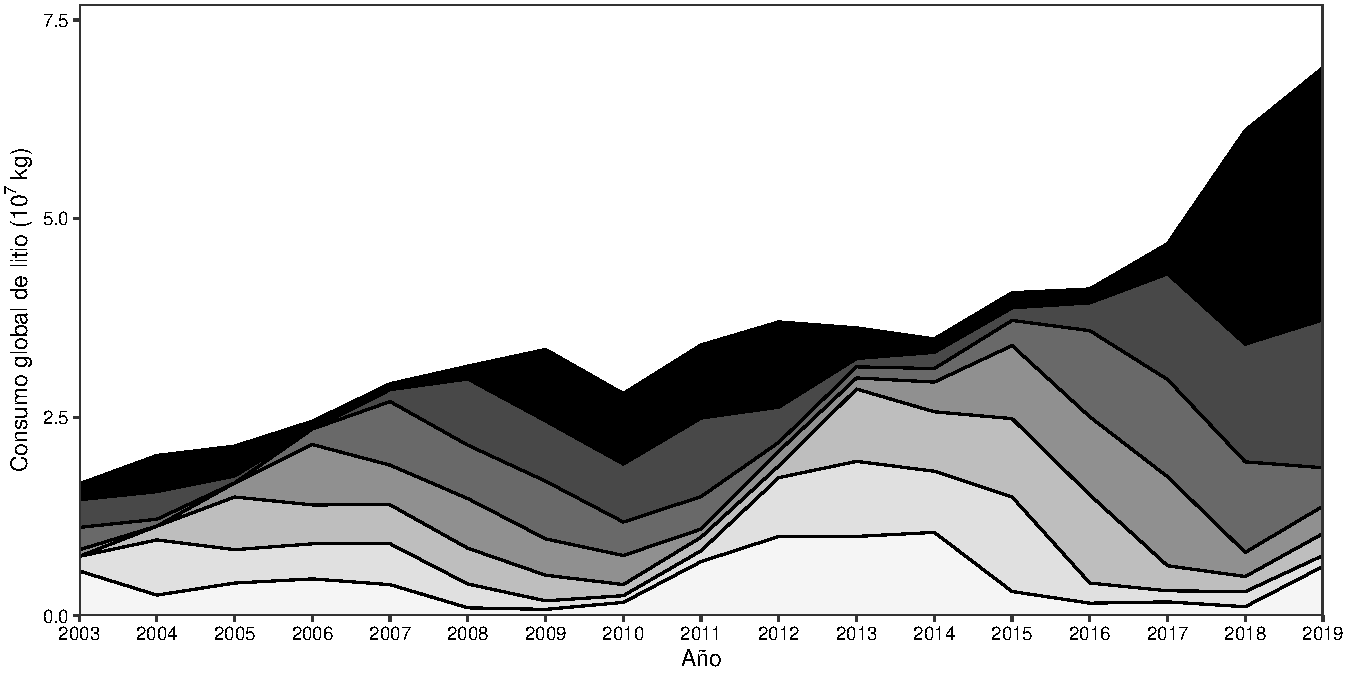
\includegraphics[width = \textwidth]{chap2/images/usesAbs.pdf}}
               \put(0, 223){\large b)}
               \end{picture}}
    \caption[Series de tiempo mercados finales de consumo de litio desde el año 2003.]{Mercados finales de consumo de litio desde el año 2003. (a) en proporción y (b) en cantidades absolutas. Las zonas del color gris más oscuro al más claro corresponden a fabricación de baterías, mejoramiento de cerámicos y vidrios, fabricación de lubricantes, síntesis de polímeros, elaboración de polvos fundentes, tratamiento de aire, y otros usos (aleaciones con aluminio, uso farmacéutico, entre otros) respectivamente.  Elaborado con datos recolectados de \citet{    SQM2003, SQM2004, SQM2005, SQM2006, SQM2007, SQM2008, SQM2009, USGS2011, USGS2012, USGS2013, USGS2014, USGS2015, USGS2016, USGS2017, USGS2018, USGS2019}.}
    \label{fig:uses}
\end{figure}

La Figura \ref{fig:uses} contiene la serie de tiempo de la evolución del mercado final del litio producido mundialmente desde el año 2003. El mercado de baterías ha monopolizado más del 60\% del consumo global de litio, que solía estar distribuido más o menos con uniformidad entre diversas industrias. En la figura con escala absoluta (Figura \ref{fig:uses}(b)), puede observarse que en los últimos años la demanda de este sector aumenta casi constantemente. Esto responde a que los humanos usamos cada vez más dispositivos portátiles que por lo general funcionan con energía almacenada en baterías de ion de litio \acused{LIB}(LIBs) y, principalmente, a la ganancia del mercado de los vehículos eléctricos \acused{EV}(EVs), en medio de la tendencia global hacia la utilización de energías y tecnologías más limpias desde un punto de vista ambiental. Adicionalmente, en algunos escenarios se especula que las baterías con litio serán la opción predilecta para almacenar energía eléctrica proveniente de fuentes renovables cuando la quema de combustibles fósiles se haga obsoleta \citep{SVERDRUP2016}.

La relevancia de este elemento ha sido reconocida por organismos gubernamentales de distintos países. La Dirección General de Desarrollo Minero de la \citet{SecEc2018} habla de la importancia de este elemento, y menciona algunos de los potenciales yacimientos que podrían posicionar al país como una potencia mundial de este recurso. El Servicio Geológico de Estados Unidos (USGS) considera que el litio es un elemento crítico que podría hacer contribuciones importantes hacia la tan anhelada autonomía energética de ese país \citep{Bradley2017}. El Servicio Geológico Británico considera al litio en su \textit{lista de riesgo} de suministro de elementos y lo ubica al mismo nivel de importancia que los metales preciosos del grupo del platino \citep{STERBA2019416}. La Unión Europea no considera al litio como un elemento crítico, pero admite que su importancia crece constantemente \citep{European2018}.

El suministro mundial de litio puede ser suficiente para varias décadas por venir, pero su futuro encarecimiento y escasez es inevitable si la flota automotriz es reemplazada en su totalidad por vehículos de propulsión eléctrica \citep{SVERDRUP2016}. Una gran parte de los análisis prospectivos que abordan la dinámica de la demanda y la oferta de metales críticos para las próximas décadas estudian el caso del litio, incluso a expensas de que algunos otros metales \textit{más críticos} están siendo ignorados en gran medida \citep{Watari2020}. Si la oferta mundial de litio llega a ser incapaz de satisfacer las necesidades del creciente sector transporte, se ralentizaría la migración masiva de este sector hacia el uso de energías más limpias \citep{VIKSTROM2013}. Algunos autores concluyen que en un futuro cercano el litio no es un cuello de botella para el suministro de las materias primas necesarias para la fabricación de \acp{LIB}, pero esto podría modificarse drásticamente obedeciendo cambios políticos o económicos que incentiven un crecimiento inesperado del sector de transporte eléctrico \citep{Olivetti2017}. En efecto, varios factores aceleran hoy por hoy el crecimiento de este sector. Un ejemplo radical lo presenta el Reino Unido de Gran Bretaña e Irlanda del Norte, cuyo gobierno ha impuesto un veto a la venta de vehículos de combustión e híbridos para el año 2035, y un veto a su circulación para el año 2050 \citep{BBC2020}.

Las \acp{LIB} son actualmente la mejor tecnología para el almacenamiento de energía eléctrica \citep{Zubi2018}. Su desarrollo entre 1970 y 1985. representó un aporte muy importante, por lo que los científicos John Goodenough, Stanley Whittingham, y Akira Yoshino fueron galardonados con el Premio Nobel de Química en el 2019 por los aportes realizados a su invención \citep{Royal2019}. Hoy en día, medio siglo después de los primeros avances en la materia, la investigación de materiales para la producción de baterías cada vez más robustas y eficientes continúa con ahínco. Por ejemplo, recientemente \citet{Harlow2019} reportaron una nueva \ac{LIB} de muy alto desempeño que podría funcionar en un auto eléctrico durante 1.6\e{6}~km, un orden de magnitud por encima de la longevidad promedio de los automóviles actuales.% Este desarrollo (patrocinado por Tesla Inc., el gigante de los autos eléctricos) ayuda a resolver uno de los mayores inconvenientes relacionados con el sector de la transportación impulsada por energía eléctrica. %\citep{Ford2012}.

% READ THIS!!!
% https://www.nobelprize.org/uploads/2019/10/advanced-chemistryprize2019-2.pdf
\clearpage
\subsection{Contexto geoeconómico}
Como en la mayoría de los elementos de la tabla periódica, la distribución del litio no es uniforme alrededor del mundo. Los mapas de las reservas y los recursos de litio por país se muestran en las Figuras \ref{fig:reservas} y \ref{fig:recursos}, respectivamente. Las reservas hacen alusión a cantidades probadas de un elemento, extraíbles de una manera económicamente viable. Los recursos hacen alusión a la estimación total de un elemento en un determinado territorio. La diferencia entre reservas y recursos viene dictaminada principalmente por la demanda de un elemento, ya que esta afecta el precio al cual se adquieren sus productos \citep{VIKSTROM2013}. 

Los mayores productores de litio actualmente son Australia y Chile. El litio de Australia es extraído de minerales que muchas veces son comercializados en forma de concentrados que requieren procesos cortos de beneficiación. Estos concentrados son usados directamente en la manufactura de cerámicos y vidrios \citep{Bradley2017}. El litio de Chile se encuentra en forma de minerales disueltos en lagos salados (i.e.\ salares).  Bolivia, Argentina y Chile son los países con los recursos de litio más grandes del mundo. Estos países definen el llamado {triángulo del litio} por la vasta cantidad de litio que tienen en sus salares. Mientras la extracción del litio de Bolivia no es viable económicamente hoy por hoy, Argentina es el cuarto productor de litio más importante \citep{USGS2020}. China tiene reservas importantes de litio y es el tercer productor más importante de este elemento. Sin embargo, el gigante asiático depende fuertemente de las importaciones debido a que por su alto nivel de industrialización consume cerca de la mitad del litio producido mundialmente cada año \citep{Olivetti2017}. 

Las reservas de litio más importantes del mundo se encuentran en los océanos, con un volumen total estimado de 1.37\e{9}~km$^3$ y una concentración promedio de litio de alrededor de 0.18~mg~kg\mnn\ \citep{KRESS20191, Evans2013, HOSHINO201311}. La cantidad de litio presente en este medio puede ser de alrededor de 250 millones de toneladas. Este valor es mucho mayor que las reservas combinadas de todos los países ricos en litio \citep{Yang2018}. En la actualidad, la extracción de litio a partir de agua de mar no es viable económicamente debido a su baja concentración y a la presencia de altos niveles de cationes que interfieren en su proceso de recobro. El costo de extracción de litio a partir de agua de mar es el más elevado y se encuentra en el extremo opuesto de una lista encabezada por el Salar de Atacama, en Chile, de donde el kilogramo de carbonato de litio equivalente\acused{LCE} (LCE)\footnote{El carbonato de litio equivalente es la terminología estándar usada en la industria del litio. 1~$kg$ de litio es equivalente a 5.323~$kg$ LCE.} se extrae a menos de 2 dólares estadounidenses (USD)\acused{USD} \citep{KUSHNIR2012}. A pesar de la no viabilidad económica de la extracción del litio presente en agua de mar, vale la pena anudar esfuerzos en el desarrollo de nuevas metodologías que permitan su recobro a partir de esta matriz porque hacia allá se puede volcar el mercado de extracción de litio cuando sus fuentes continentales, más rentables y menos complicadas, empiecen a escasear.

El precio de los compuestos principales de litio ha aumentado casi constantemente en los últimos años \citep{MARTIN2017}. En el 2019, en medio de la guerra comercial entre China y Estados Unidos, China redujo los generosos subsidios que estaba otorgando a compradores y fabricantes de \acp{EV} y esto produjo una sobreoferta de litio que repercutió en una disminución de su precio en casi un 25\% \citep{Kalantzakos2019}. Sin embargo, la popularidad de los \acp{EV} sigue en aumento, y la balanza de la oferta-demanda podría inclinarse nuevamente a favor de los países productores de litio en cualquier momento \citep{LIU2019}.

%https://sci-hub.tw/10.1016/j.watres.2019.01.050

% https://sci-hub.tw/10.1016/j.apenergy.2013.04.005

\begin{figure}[H]
    \centering
    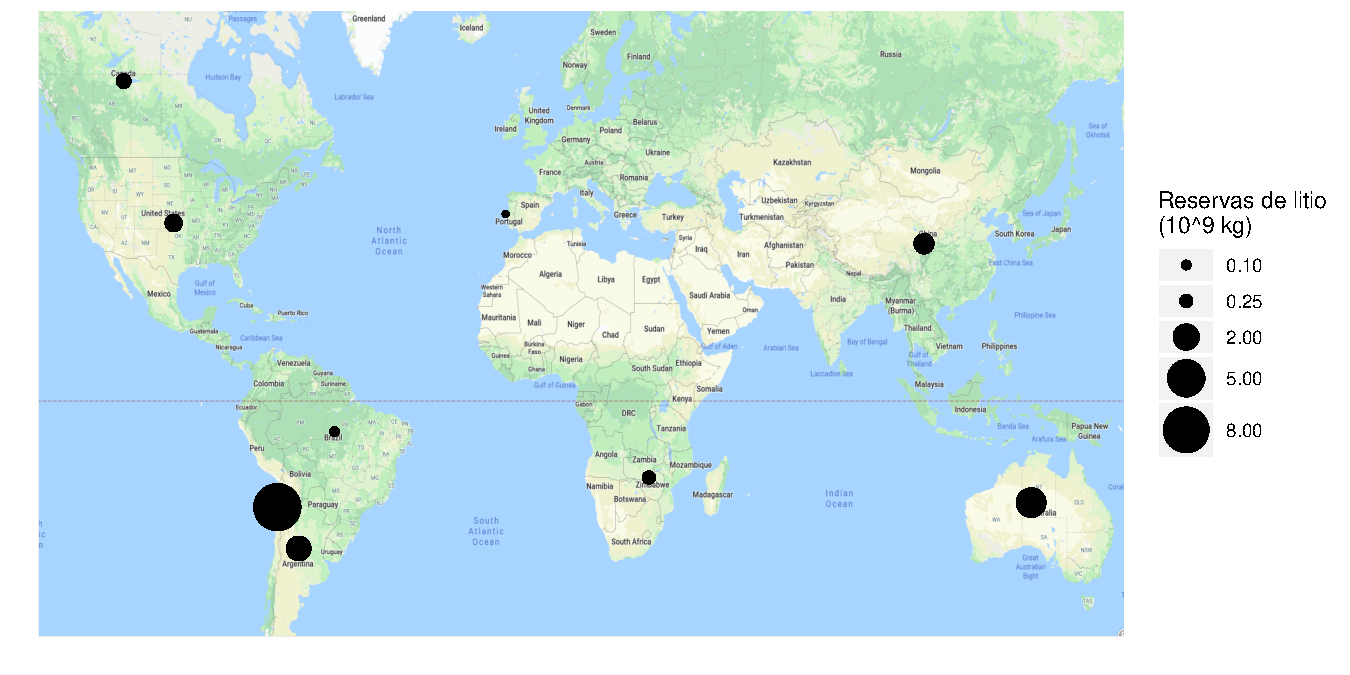
\includegraphics[width = \textwidth, trim = {1cm 1.2cm 0.4cm 0.5cm}, clip]{chap2/images/reserves.pdf}
    \caption[Reservas de litio por país.]{Reservas de litio por país. El diámetro de los círculos es proporcional a la cantidad de litio en millones de toneladas \citep{USGS2020}.}
    \label{fig:reservas}
\end{figure}
\begin{figure}[H]
    \centering
    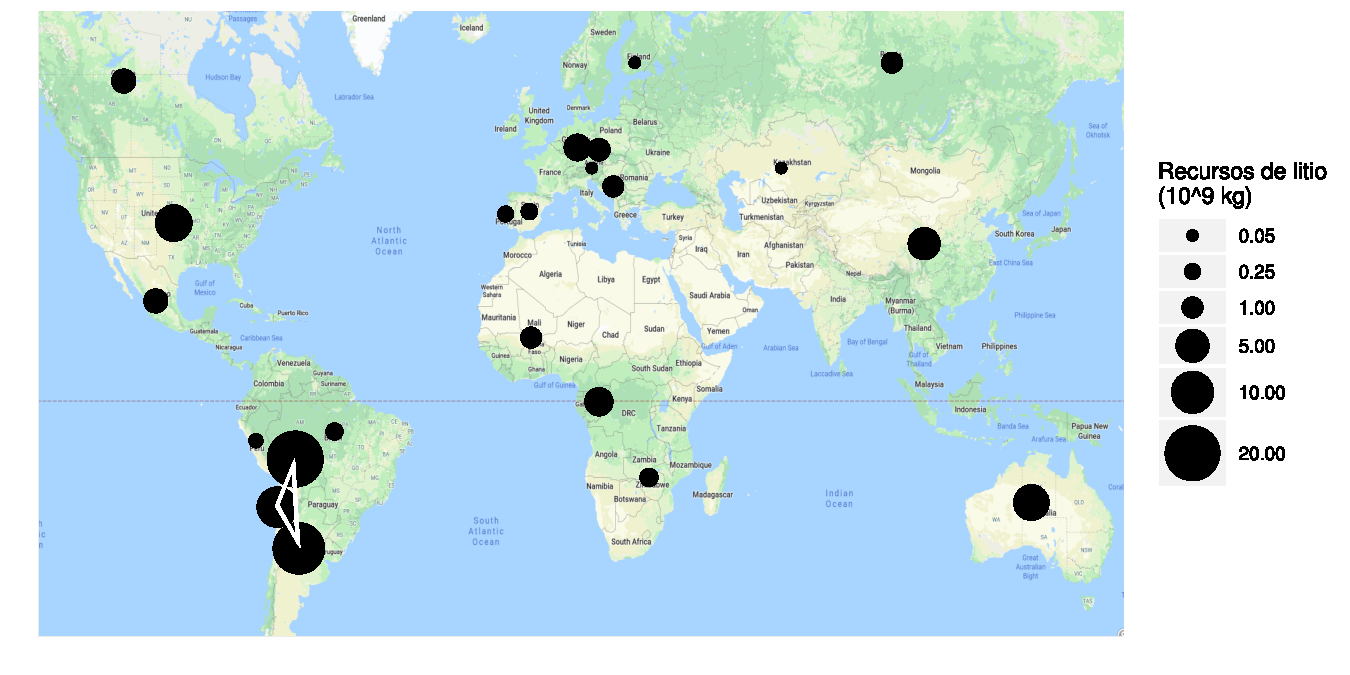
\includegraphics[width = \textwidth, trim = {1cm 1.2cm 0.4cm 0.5cm}, clip]{chap2/images/resources.pdf}
    \caption[Recursos de litio por país.]{Recursos de litio por país. El diámetro de los círculos es proporcional a la cantidad de litio en millones de toneladas \citep{USGS2020}. El {triangulo del litio} en Suramérica se señala con blanco.}
    \label{fig:recursos}
\end{figure}

\subsection{El litio de México}\index{Litio!Bacadéhuachi-Sonora}
%https://www.gob.mx/cms/uploads/attachment/file/419275/Perfil_Litio_2018__T_.pdf
%https://www.bacanoralithium.com/pdfs/Ni-43-101-Mineral-Resource-Estimate-For-The-Sonora-Lithium-Project-Mexico-May-2015.pdf
%https://www.bacanoralithium.com/pdfs/Bacanora-FS-Technical-Report-25-01-2018.pdf
México no figura entre los grandes productores de litio. Como puede observarse en la Figura \ref{fig:reservas}, el Servicio Geológico de Estados Unidos no contabiliza reservas en este país. % y la Figura \ref{fig:recursos} muestra que los recursos que le atribuyeron a México no llegan a las dos millones de toneladas. 
No hay proyectos de litio en fase de explotación comercial en territorio mexicano y las importaciones de este elemento involucran un negocio multimillonario que se encuentra exento de pagos arancelarios \citep{SecEc2018}. A pesar de esto, en un futuro cercano México podría sentarse en la mesa de las potencias del litio.

Se encuentran en etapa de exploración cerca de 11 proyectos de extracción de litio, de los cuales el más importante se encuentra en Bacadéhuachi, en el estado de Sonora, al norte del país. La locación se atribuye ser actualmente el proyecto de explotación de litio más grande del mundo, con una exorbitante cantidad de más de 240 millones de toneladas de mineral con una concentración promedio de litio de 0.35\% en masa \citep{Bacanora2018}. Esta cifra ha sido muy mal utilizada por la prensa común, que irresponsablemente habla de {240 millones de toneladas de litio}.\footnote{Esto es equivalente a la cantidad total de litio presente en la vastedad de los océanos, el mayor reservorio de litio de nuestro planeta.} Esto puede conducir a la errónea conclusión de que México es la nueva Arabia Saudita del litio. La estimación real en el yacimiento es de cerca de un millón de toneladas extraíbles a un excelente costo total de producción de aproximadamente 4 \ac{USD}~kg$_{LCE}^{-1}$. Estas cifras son bastante prometedoras, y ubican al país como el cuarto o quinto con las mayores reservas de litio en el mundo. El yacimiento consta principalmente de arcilla de hectorita (ver Sección \ref{sec:arcillas}). Ya se encuentra en operación una planta piloto de refinamiento y purificación para la obtención de carbonato de litio de grado para baterías ($\geqslant$99.5\%). Se espera que la mina entre en operación en el 2022 \citep{Bacanora2018}.

% Tesla y Bocanora firmaron convenio para asegurar el suministro de litio al gigante de los EVs

%La zona del yacimiento de litio de Bacadéhuachi-Sonora es actualmente azotada por violencia de los carteles de narcotráfico y se le considera una región inestable. Resulta inevitable rememorar  los yacimientos de oro en el norte del País y el contexto de la fiebre del oro de California en la época de la injusta guerra México-Estados Unidos que cambió tan drásticamente el mapa de Norteamérica. Los tiempos han cambiado desde entonces. Casualmente, el litio ha sido denominado por muchos como oro/petroleo blanco \citep{Crooks2018} y el hecho de que el yacimiento se encuentre \textit{tan lejos de Dios y tan cerca de los Estados Unidos} (a menos de 300 km de la frontera México-Estados Unidos) puede tener poco que ver pues atravesar el océano atlántico no fue inconveniente para los Estados Unidos en el conflicto bélico con (su ex-aliado) Irak en la Segunda Guerra del Golfo para ocupar su territorio y disponer de sus recursos bajo un pretexto que nunca pudo ser demostrado. Sin embargo, una posible invasión suena muy inverosímil y los amados del neoliberalismo tienen herramientas más sutiles para despojar de sus recursos a los países que despectivamente han denominado \textit{tercermundistas}. El Gobierno de México debe pensar al respecto con calma y aparte de recordar siempre su historia para no tener que repetirla, puede aprender de algunos de los muchos errores de su \textit{Aliado del Pacífico},\footnote{La Alianza del Pacífico es un acuerdo de cooperación multilateral establecida en el 2011 por Chile, Colombia, México y Perú. El propósito es prosperar juntos y crear un bloque latinoamericano competitivo frente al mundo \citep{Prado2016}.} el Gobierno Colombiano, y evitar un detrimento irremediable de su Patrimonio Nacional.\footnote{En el año 2000, el Gobierno de Colombia vendió (regaló) su participación en la mina de carbón térmico bituminoso de alta calidad más importante de Latinoamérica, El Cerrejón. El evento coincidió con un alza pronunciada en el valor comercial de este recurso. Mientras en la zona de la mina se presencia pobreza extrema y un medio ambiente sumamente deteriorado, cada 4 horas salen locomotoras con más de $10^7$ kg de carbón que es vendido al mejor postor por parte empresas extranjeras que supieron, en el momento correcto, manipular y comprar a políticos endebles y corruptos que abundan en ese país sudamericano.}


%\subsection{Propiedades químicas}
\subsection{Principales fuentes de litio}\index{Litio!fuentes}
Las principales fuentes de litio, sus compuestos más comercializados y el uso más común de los mismos se muestran en la Figura \ref{fig:esquemaSpiers}. Como se mencionó anteriormente, las reservas son fuentes extraíbles con procesos económicamente viables y los recursos incluyen todas las fuentes del elemento a pesar de la inviabilidad práctica de su extracción. A pesar de que el litio se encuentra presente en minerales, salmueras, arcillas y (principalmente) en agua de mar, la extracción a gran escala solo se hace actualmente partir de minerales (rocas), y salmueras. Con el éxito de las minas como las de Sonora en México, las arcillas pueden pasar formar parte importante de las fuentes comerciales de este elemento. Ya se encuentran en operación plantas piloto para la producción de carbonato de litio a partir de arcillas y producen litio a precios muy competitivos \citep{Bacanora2018}.

Los procesos extractivos industriales pueden compartir características generales para fuentes de la misma naturaleza, pero las metodologías aplicables a un determinado yacimiento dependen en gran medida de las particularidades que presentan los recursos de dicho yacimiento. De esta manera, un proceso hidrometalúrgico diseñado para extraer litio de un salar en China puede no funcionar apropiadamente si se aplica sin modificaciones importantes a la extracción de litio de un salar en Bolivia.

{\floatstyle{boxed}
\restylefloat{figure}
\begin{figure}[H]
    \centering
    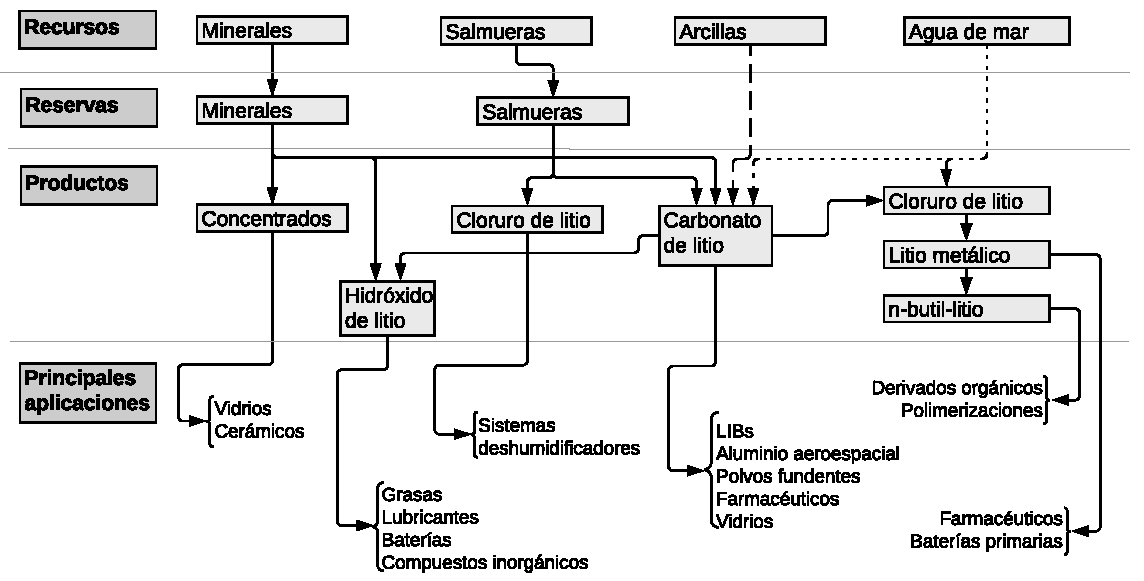
\includegraphics[width=\textwidth]{chap2/images/lithiumsoourcetoeum.pdf}
    \caption[Principales rutas del litio desde la fuente hasta su uso final.]{Principales rutas del litio desde la fuente hasta su uso final. Adaptado principalmente de \citet{SPEIRS2014}. La línea discontinua que desprende de arcillas es considerando el éxito de de proyectos como el de Bacadéhuachi-México y las líneas punteadas que desprenden de agua de mar son considerando la posible aplicación del presente proyecto.}
    \label{fig:esquemaSpiers}
\end{figure}
}

\subsubsection{Minerales en roca}\label{sec:pegma}
Los minerales de litio más relevantes se muestran en la Tabla \ref{tab:minerals} \citep{Anthony1995}. Estos minerales se presentan por lo general en forma de pegmatitas.\footnote{Rocas ígneas filolianas con intrusiones cristalinas} Las pegmatitas constituyen actualmente la mayor fuente de litio. Las minas más grandes de pegmatitas con litio están localizadas en Australia. La extracción del litio presente en esta matriz requiere inicialmente la destrucción del mineral por métodos mecánicos o químicos que demandan mucha energía y con frecuencia aumentan el costo de la extracción \citep{CHRISTMANN2015}.

\begin{table}[h]
    \centering\footnotesize
    \begin{tabular}{@{}llrp{7cm}@{}}\toprule
        \textbf{Mineral} & \textbf{Fórmula empírica} & \textbf{Li (\%)} & \textbf{Detalles} \\\midrule
        Espomudena & \ce{LiAl(SiO3)2}      & 3.73 & Principal fuente mineral de litio.\\
        Lepidolita & \ce{KLi2AlSi4O10F(OH)}& 3.58 & Mineral de litio más abundante. Segunda fuente mineral más importante.\\
        Petalita   & \ce{LiAlSi4O10}       & 2.09 & Puede convertirse en Espomudena de alta calidad para su uso directo en cerámicos.\\
        Ambligonita& \ce{Li_{0.75}Na_{0.25}Al(PO4)F_{0.75}(OH)_{0.25}} & 3.44& Algunos yacimientos presentan hasta 10\% en masa de litio pero no es una fuente comercial importante por su baja abundancia.\\\bottomrule
    \end{tabular}
    \caption{Principales minerales (en roca) de litio.}
    \label{tab:minerals}
\end{table}

El mineral más importante de esta familia es la espomudena, cuyos concentrados pueden ser utilizados directamente como aditivo en vidrios y cerámicos, el segundo mercado final más importante del litio. Los concentrados son el resultado del beneficio de los minerales. En este caso, el beneficio puede ser realizada por medios mecánicos como flotación con líquidos densos y separación magnética \citep{TADESSE2019}. 

Para obtener compuestos de litio, el concentrado de mineral debe ser {tostado} a altas temperaturas en presencia de algún aditivo para formar compuestos lixiviables. Posteriormente el litio se concentra con resinas de intercambio iónico. Si se usa como aditivo, por ejemplo, ácido sulfúrico, se forman sales de sulfato que son lixiviables con agua caliente. Al elevar el pH del lixiviado acuoso, se eliminan por precipitación una parte importante de los cationes interferentes. La carbonatación de la disolución produce carbonato de litio, el compuesto más comercial de este elemento \citep{TRAN2015}.

\subsubsection{Salmueras}
Las salmueras de los salares componen actualmente los recursos más abundantes de litio. Los lagos salados con mayor cantidad de litio se encuentran en el triángulo del litio (ver Figura \ref{fig:recursos}), formado por Bolivia, Argentina y Chile. La concentración de litio en las salmueras de importancia comercial se encuentra entre 200 y 4000~mg~kg\mnn. La extracción del litio presente en estas matrices presenta la ventaja de que el elemento ya se encuentra en disolución y ya no son necesarias algunas de las etapas que consumen más energía cuando el litio se extrae a partir de minerales sólidos.

La obtención de compuestos de litio requiere inicialmente la eliminación de una porción importante del disolvente (agua), para concentrar el litio en el medio. Usualmente esto se hace por evaporación solar o por ósmosis inversa \citep{Swain2017}. El protocolo empleado en cada salmuera es diferente porque depende de las características del yacimiento. Si la salmuera contiene boro, este por lo general se retira con extracción por disolventes, porque el ácido bórico es un subproducto con valor comercial y porque el boro daña los sistemas de obtención de litio metálico a partir del cloruro de litio \citep{TRAN2015}. Los iones calcio y magnesio deben ser retirados por preci\-pi\-tación y posteriormente puede carbonatarse la disolución para precipitar carbonato de litio que posteriormente es purificado por recristalización o por filtración.

\subsubsection{Minerales en arcilla}\label{sec:arcillas}
Las  arcillas no son actualmente una fuente importante de litio, pero la situación promete cambiar próximamente con el avance de megaproyectos mineros ubicados principalmente en México y Estados Unidos. Las arcillas de litio más representativas se muestran en la Tabla \ref{tab:clays}. La más importante de este grupo es la hectorita. El proceso de extracción de litio a partir de estas matrices es similar al aplicado para obtener compuestos de litio a partir de rocas pegmatiticas.

\begin{table}[H]
    \centering\footnotesize
    \begin{tabular}{@{}llr@{}}\toprule
        \textbf{Mineral} & \textbf{Fórmula empírica} & \textbf{Li (\%)}\\\midrule
        Hectorita & \ce{Na_{0.3}(Mg,Li)_3Si_4O_{10}(OH)_2}  & 0.54 \\
        Jadarita & \ce{(Na,Ca)_{0,3(}Al,Mg)_2Si_4O_{10}(OH)_2.n(H_2O)}& -\\
        Polilitionita   & \ce{KLi_2AlSi_4O_10(F_{0.75}(OH)_{0.25})_2}       & -\\\bottomrule
    \end{tabular}
    \caption{Principales minerales (en arcillas) de litio.}
    \label{tab:clays}
\end{table}

El proceso de benefio de las arcillas involucra un proceso de molienda fina y clasificación por tamaño de partícula usando un hidrociclón. Los aditivos añadidos en el tueste del concentrado son principalmente sulfato de sodio, sulfato de calcio (yeso) y carbonato de calcio (calcita). Se produce sulfato de litio que puede tratarse como se describió en la Sección \ref{sec:pegma} \citep{Bacanora2018}. Como subproducto de valor comercial se suele obtener sulfato de potasio.

\subsubsection{Agua de mar}
El litio se encuentra disuelto en el agua de mar a una concentración promedio de 0.18~mg~kg\mnn\ \citep{Evans2013}. Su concentración es diminuta, pero es el decimocuarto elemento más abundante en esta matriz. Como se ha mencionado en secciones anteriores, los océanos contienen el recurso de litio más grande conocido del planeta, y constituyen una fuente casi inagotable de este elemento \citep{Yang2018}; sin embargo, su extracción a escala industrial es inviable económicamente a causa de su baja concentración. Distintas metodologías son estudiadas actualmente para extraer litio a partir de esta matriz, pero se encuentran en etapa de investigación y desarrollo, por lo que se han incluido en la Sección \ref{sec:estadodelarte}.

\subsubsection{Reciclaje}

Actualmente, las cantidades de litio obtenidas por reciclaje no son importantes y puede que este panorama no cambie en un futuro próximo \citep{Olivetti2017}. El litio utilizado en cerámicos y vidrios no se puede recuperar \citep{CHRISTMANN2015}, y la minería urbana de \acp{LIB} por lo general se enfoca en la recuperación de cobalto o manganeso que tienen un mayor valor comercial. 

Algunas estimaciones establecen que para el 2050 el 25\% de la producción mundial de litio podría provenir de fuentes recicladas involucrando principalmente \ac{LIB}s. Este aumento del porcentaje sería en respuesta a la introducción al mercado masivo de baterías de litio de gran tamaño para \ac{EV}s, con el consecuente gran volumen de residuos que pueden representar dichas baterías hacia el final de su tiempo de vida útil (cerca de una década) \citep{STERBA2019416, Evans2013}. Predicciones sobre el crecimiento de la flota de vehículos eléctricos estiman que tan solo en los Estados Unidos podrían producirse hasta cuatro millones de toneladas de residuos de \ac{LIB}s en las próximas dos décadas \citep{RICHA2014}. 

Las \ac{LIB}s tienen entre 100 y 345~g de litio por cada kilowatt hora de capacidad. Esto representa cerca de 4~kg de litio en la batería de cada \ac{EV}. La dificultad principal que presenta el reciclaje del litio de estas fuentes recae en que la química de los cátodos empleados es muy variada (Tabla~\ref{tab:catodos}), y la minería urbana de este recurso se puede hacer menos eficiente dado que cada material requiere condiciones distintas de tiempo y composición, para la lixiviación eficiente de litio \citep{VENKATRAMAN2004}.% Políticas estrictas deberán establecerse para regular la recolección y clasificación de las baterías que han terminado su ciclo de vida.
\begin{table}[H]
    \centering\footnotesize
    \begin{tabular}{@{}p{3cm}lcp{5cm}@{}}\toprule
        \textbf{Nombre} &\textbf{Fórmula} &  \textbf{Energía específica}&\textbf{Detalles}\\
        &&(W~h~kg\mnn)\\\midrule
        Óxido de litio y cobalto (LCO) & \ce{LiCoO2} & 110-200 & Primer cátodo de uso industrial en \ac{LIB}s. Presenta desventajas de seguridad y ambientales, por riesgo de explosión y por el uso de cobalto, respectivamente.\\
        Óxido de litio, niquel, manganeso y cobalto & \ce{Li(Ni_{0.33}Mn_{0.33}Co_{0.33})O2} & 95-130 & Amplio uso en vehículos eléctricos.\\
        Espinela de litio y manganeso & \ce{LiMn2O4} & 110-120 & Bajo costo de producción. Amplio uso en vehículos híbridos eléctricos.\\
        Fosfato de litio y hierro & \ce{LiFePO4} & 95-140 & Es de los cátodos más seguros, con los menores costos de producción y con un bajo impacto negativo al medio ambiente\\\bottomrule
    \end{tabular}
    \caption[Principales materiales de los cátodos de LIBs.]{Principales materiales de los cátodos de \ac{LIB}s \citep{Chagnes2015}}
    \label{tab:catodos}
\end{table}

\subsection{Problemas socio-ambientales asociados}
El litio permite el funcionamiento de diversas tecnologías que prometen ayudar a disminuir el impacto ambiental negativo que acarrean muchas de las actividades humanas. A pesar de esto, su extracción y utilización no está libre de consecuencias para algunos de los ecosistemas y las poblaciones que rodean los yacimientos importantes.

El ejemplo más notorio lo presenta la extracción del litio presente en el Salar de Atacama en Chile, parte del triángulo del litio. La evaporación de grandes cantidades de agua de los salares para aumentar la concentración de litio resulta catastrófica para la fauna del lugar, porque el Desierto de Atacama es un lugar extremadamente seco y el acceso a las fuentes hídricas se encuentra injustamente restringido a su aprovechamiento comercial. Los reservorios subterráneos de estos salares son alimentados por fuentes acuáticas que también alimentan lagos que son muy importantes para las regiones circundantes. La minería de litio en esta región compite con los pobladores por el uso del agua y en los últimos  censos nacionales se ha evidenciado una caída importante en su población \citep{Romero2012, LIU202012}.

Por otro lado, el Salar de Uyuni, en Bolivia, es el segundo reservorio más grande conocido de litio (después de los océanos) con una excepcional estimación de 20 millones de toneladas de litio. Una dificultad importante que presenta la extracción de litio de este salar es que el ecosistema es muy delicado y el proyecto representaría una amenaza importante a la biodiversidad de la zona \citep{Hancock2018}. La protección de las especies endémicas de la región y de los pueblos indígenas que habitan la zona son un factor importante que afortunadamente han ralentizado el inicio de la explotación de este recurso.

Cuando la extracción de litio se hace a partir de rocas y arcillas, los procesos de calcinación y tueste tienen un gran impacto negativo al ambiente porque demandan altas cantidades de energía, liberan grandes volúmenes de emisiones atmosféricas, e involucran el uso de grandes cantidades de ácido \citep{Hancock2018}.

Los problemas sociales y ambientales de la extracción de litio a partir de agua de mar pueden ser significativamente menores que los asociados a los procesos de recobro a partir de salmueras y minerales rocosos o arcillosos. La cuasi-omnipresencia de los océanos permitiría ubicar los puntos de extracción en lugares donde el ecosistema sea robusto y no haya afectación a poblaciones humanas.

Respecto a los productos finales de litio, la fabricación de una batería con 1~kWh de capacidad requiere la inversión de cerca de 380~kWh de energía y el proceso puede liberar hasta 80~kg de \ce{CO2} \citep{Chagnes2015}. Al final de su ciclo de vida, estas baterías son consideradas residuos peligrosos que representan un peligro para el medio ambiente y para la salud de los humanos debido a sus altos contenidos de cobre, cobalto y níquel \citep{Kang2013}. El impacto negativo de estos residuos se mitigaría considerablemente con la implementación de políticas estrictas referentes al reciclaje de estos recursos.
